\newpage
\pagenumbering{arabic}
\section{INTRODUCTION} 
\subsection{Background of the Study}
Representative governments, be in parliamentary or presidential system of representation, are accountable to the public welfare of the citizens. Autocratic and dictatorial regimes also heed the needs of people even though there is no direct accountability\cite{Gilli2014} through elections or other measures. The economic blueprint of a nation is largely shaped by the political and institutional factors, which are reflected in the fiscal performance at the national and subnational level\cite{Rattso1998, Dafflon2002}. Subnational government could take various forms, some having only deconcentrated and delegated power while others possessing decentralized structure where powers, specifically economic, political, and fiscal powers are factually devolved to the subnational levels. It should be noted that decentralization, inherently, is neither good nor bad for efficiency, equity, or macroeconomic stability, rather its effects depends on institutional specific design and how building block of fiscal federalism namely, expenditure and revenue assignments, intergovernmental transfer, and subnational borrowing processes, are designed\cite{Alt1994}. \\
Since subnational government play a crucial role in the overall economic development of nations, several studies have examined subnational government efficiency and its major determinants\cite{Deborger1994, Worthington2000, Geys2006, Bruns2008}. Subnational government are designed to be closer to people and has the motive to increase public welfare, thus it is hard to develop a performance metrics to objectively measure and judge them\cite{Gray2006}. However, economic literature provides several methods through which it could be reasonably done and fiscal performance is one of such chief metrics. Different countries have different reasons to decentralize or devolve real powers, and procrustean model of power sharing, without regard to the reasons for the creation of federal structure, are destined to fail. Diversity in geography, economic status, language, and natural and human resources meant that different regions of Nepal had varying levels of needs and types of government services. The desire of people, the electorate, to better access and be involved in the governing mechanism, along with bevy of other factors,  drove out the largely-autocratic and centralized rule of monarchial system and instituted Nepal as a Federal Republic.\\
The constitution of Nepal, formally promulgated in 2015, mandated Nepal to have a federal republic system of governance. Under this system, Nepal is administratively divided into 753 local levels, 7 provinces, and a unitary central government. The constitution also delineated the jurisdiction of each of these three levels of government, from the revenue and expenditure assignments of each levels to the inter-relationship among them. The vestige of old administrative system before the initiation of federalism still remains; explicitly in some cases, with the 77 district still holding considerable authority; or implicitly in other cases , with the new local level and province level boundary closely resembling the old Municipalities(or V.D.Cs.) and the development regions respectively. The installation of federalist structure, with considerable power devolved from the central to especially the local level governments could be thought of as another effort to development in the changed political and socio-economic context of Nepal. Federalism with a proper decentralization of power is assumed to be helpful not only for economic growth of the local levels\cite{Iimi2005,Sasana2019,Carniti2019},  but could also aid in reducing inequality in development across federal regions\cite{Baskaran2016}. Beyond economic growth, Federalism, with sufficient fiscal and economic authority decentralized with proper accountability mechanism, can help improve the democratic system of governance and can also assist in removing several impediments to development\cite{Weingast2014}.\\
However, federalism is not a universal panacea for economic growth and development. Federalism, as a doctrine of governance, does not have a standardized format and differs in the way it is implemented across countries and across time. Moreover, there are countries, like the USA, that were initially formed with a federal structure\cite{Sargent2012}, whereas others, such as Nepal, adopted federalism long after their formation. Additionally, federal system across nations were generally instituted more on the rational of political considerations rather than of economic welfare\cite{Riker1964}.  Thus, Federalism should be considered from multiple perspectives with economics as a key aspect, but not the only one. Furthermore, federalism can be ill-suited  when dealing with economic as well as other crises and long-run stability\cite{Huberfeld2020}. \citeA{Peterson1995} in his seminal work, \textit{The Price of Federalism}, argues that for federalism to  work, its functional and legislative perspective must be smooth and in tandem, and any discrepancies between these two perspectives would render federalism unsuitable as the governance mechanism.  \\
Against such backdrop, Nepal instituted federalism through the constitution, with political, fiscal, economic, and other powers devolved and decentralized from the central unitary government to province and local-level governments\footnote{The brief overview on the number of federal structures is shown in Table 1}. While all local level governments wield considerable administrative power, not all local levels were created equal. These inequalities are reflected not only in demographic and geographic aspects, but also in the level of development as well as in the revenue and expenditure mobilization aspects of the local levels. In demographic aspect, Narpa Bhumi in Manang harbors the population of 538, while Kathmandu metropolitan city houses 862,400 people.\hspace{1mm}Similarly, Bhaktapur municipality is the smallest local level with area of 6.56 sq.km.\hspace{1mm}while Namkha rural-municipality in Humla district is largest with the area of 2419.64 sq.km.. \\

\begin{table}[H]
  \centering
   \begin{tabular}{lcccc}
    \hline
    \multirow{2}{*}{Province} &\multicolumn{4}{c}{Numbers of Local Levels}\\ & \multicolumn{1}{c}{$Rural-Municipalities$} & \multicolumn{2}{c}{$Municipalities$}  & \multicolumn{1}{c}{$Sub-Metros \& Metropolitans$}\\
        \hline
    Koshi & 88 && 46   & 3 \\
    Madhesh & 59 & & 73 & 4 \\
    Bagmati & 74 & & 41& 4\\
    Gandaki &58 & &26 &1\\
    Lumbini & 73 && 32  & 4\\
    Karnali & 54& & 25   & 0\\
    Sudurpaschim & 54& & 33  & 1\\
    \hline
    Total & 460  && 276 &  17\\
    \end{tabular}
    \caption{Province-wise local levels classification}  
     \label{Province-wise local levels classification}
\end{table} 
 
The advantages of federalism, namely, aiding in economic growth, reducing inequality, and strengthening democratic system of governance stem primarily because of the federal units having better understanding of and being more responsible to the demands of its denizens. Since 1980s, power devolved structure of governance, like federalism, has emerged as a valued political and economic goal in most developing countries, with advocates of such devolution justifying it on grounds of increased efficiency, more thoroughgoing equity, and for greater participation and responsiveness of government to citizens\cite{Agrawal2000}.  \citeA{North1981} explains how the state, an entity with comparative advantage in violence, realized its constraints as it grew in geography and population, and instituted the \emph{bailiff} system, a historical precursor of the modern federal system. In the bailiff system, in which the sub-state units, by design were closer and more responsible to their denizens, a central ruler would install local rulers who were permitted to have their own bureaucracy, but still exerting stringent monitoring and controls over their actions.\\
 The modern day federalism retains many characteristics of the bailiff system, although the desideratum motive in federalism is not the constraints on the central state's capacity but the democratic ideals of proper representations and responsibilities in governance. Devolving powers to subnational units creates the realm of decision making where those subnational units, or federal units, can exercise some autonomy while addressing the needs of the local populace. In democracy, voices of all denizens must be heard and sometimes it could result in `tyranny of majority' where the voices and opinions of the minority group are not addressed properly. Federalist structure of governance addresses this issue as federal units, being smaller than the national government and being closer to the people, could represent the interest of people better. It is particularly useful when there exists uneven state of development within the nation, as federal units could tailor the policies to properly address the exact needs of the people. This view of federalist structure tailoring policies to better address the needs of the local region was succinctly summarized by Justice Brandeis, as :``It is one of the happy incidents of the federal system that a single courageous state may, if its citizen choose, serve as a laboratory, and try moral, social, and economic experiments without risk to rest of the country"\cite{Rosen2016}. \\
Federal units, being closer to the denizens and thus, more knowledgable to properly tailor policies for better addressing the local needs, benefit other units and nations as a whole as it would create stronger links of political accountability among local governments, the central government,  the public sector, and the community\cite{Eckardt2008}. \citeA{Agrawal2000} points out that along with representation, accountability is critical if devolved powers are to serve local needs efficiently and equitably. Thus, in federalism, the subnational units are important not just because they represent local people and their demands, but also because they are accountable to the local people. In Eckardt's model of decentralization, there exists three distinct dimensions underlining all acts of decentralization, namely, actors. powers, and accountability. For federalism to attain its political and economic goals, there needs to be an understanding of the powers of various actors, the domains in which they exercise their powers, and to whom and how are the actors accountable. In democratic nations, such actors are mostly held downwardly accountable to local/federal constituencies, mainly through the electoral processes. \citeA{Blair2000} states how democratic local governance works primarily through participation and accountability. Participation, in this context, means giving meaningful role to citizens on decision that affects them, while accountability aspect is twin-fold, with bureaucrats accountable to elected officials and elected officials accountable to the local public. Such accountability is carried out through the working of four mediums, namely, elections, political parties, civil society, and media. \citeA{Przeworski1999} states that since the establishment of representative institutions, be it at national or subnational level, their basic structure has largely been; 
\begin{enumerate}[label=\roman*.]
    \item Rulers who govern are selected through the electoral processes. 
    \item Citizens, who vote and can urge rulers to follow a set of mandates but can't give legally binding instruction during the rulers' tenure.
    \item Rulers are held accountable through periodic elections where citizens vote.
\end{enumerate}
Economic and public choice literatures assume that voters involvement, which can be measured through electoral participation enhance accountability and discourage rent seeking as well as shirking behavior, thereby increasing efficiency and other aspect of governance\cite{Stigler1972, Barro1973}. 
Thus, election acts as the accountability mechanism that connects citizens with their representative. The primary motive through which election fulfills its role in making leaders accountable is through the anticipation of not being reelected in the future leads the leaders not to shirk their obligations to voters in the present\cite{Barro1973, Ferejohn1986, Manin1997}. \citeA{Fearon1999} describes two principal mechanism by which elections might bring about public policies that voters desire - sanctioning and selection, Sanctioning mechanism works as elected officials are motivated to choose policies that most of the voters desire so as to get reelected, and selection mechanism work as voters usually have the options to select other opposition candidates who they could be better and less likely to shirk from their responsibilities.\citeA{Besley2002} finds that in India, state governments are more responsible to local needs, especially in public service distribution during the time of emergencies, calamities, and disasters , where electoral accountability is greater.\\
Periodic election is the sin-qua-non feature of democracy. Elections provide mandates to the elected officials and give the people their say on organization of all aspect of the nation. One of the core feature of the modern day federalism is selections of federal legislatures and executives by the denizens of the federal units through periodic elections. As fiscal and economic power devolution are usually carried out, the elected leaders of the federal units are accountable to the public for the fiscal and economic health of the federal units. Through sanctioning and selecting mechanisms, the incumbent elected officials are motivated to improve the fiscal and economic indicators. Much of the research and literature on fiscal federalism reflects the traditional public finance approach to the issue\cite{Galligan1990}, which was driven by the Musgravian principles of efficiency, equity , and stability\cite{Musgrave1983}. Even in the Musgravian approach to fiscal federalism, periodic elections for the rulers is the critical component of the well-designed power devolution system.  \\
Accountability mechanism functions as a map from outcomes of actions of public officials to sanctions by citizens. Elections are a ``Contingent renewal" of accountability mechanism, where sanctions are to extend or not to extend the governments' or incumbents' tenure\cite{Przeworski1999}. However, bridging accountability aspects of leaders towards fiscal and economic responsibilities with electoral motivations is not straightforward. One of the critical methodological roadblocks in conducting research of fiscal and economic performance is that no exact or well agreed performance metrics of public sector exists\cite{Estrella2003, Andrews2003, Uphoff2005}. In private sectors, the economic roles and objectives are usually clearly outlined, making performance measurement and inference easier. Compounding the problem of accountability aspect is the informational aspects, especially as there exists informational asymmetry between elected officials and the voters. For example, elected officials might be more tempted by long run capital investment projects which are ultimately beneficial to the public but it incurs costs in the long run, thus, it creates a healthy fiscal result in the long run but public might be dismayed by the short term fiscal and economic costs. Additionally, when the incumbent expects that he or she will not be reelected, then it could result in the incumbent choosing not to be accountable and to extract high rents, breaking down the voters control completely\cite{Ferejohn1986, Banks1998}.   \\
After the promulgation of the constitution, Nepal conducted its first election in a newly delineated local level in 2017 in three distinct phases. The differences in local levels was reflected in the voting turnout as well as in the electoral competition, as seen in Figure \ref{Heatmap of Voting turnout} and Figure \ref{Heatmap of HH index} respectively. The initial differences in local level entities have other implications too, as more populated local level getting more funds from the central and provincial government as the population is one of the key factor in grants consideration\footnote{NNFRC Fiscal Equalization Grant to local level criteria includes formula-based, minimum, and performance-based grants, all influenced by total and dependent population size.}. Most importantly, after the promulgation of the constitution and two local-level election cycles concluded, some local levels have achieved considerable improvement in development while some have lagged behind\footnote{NNFRC annual reports as well as available provincial reports from Provincial Planning Commissions}. 
\begin{figure}[hptb]
\centering
\hspace{-1.2cm}
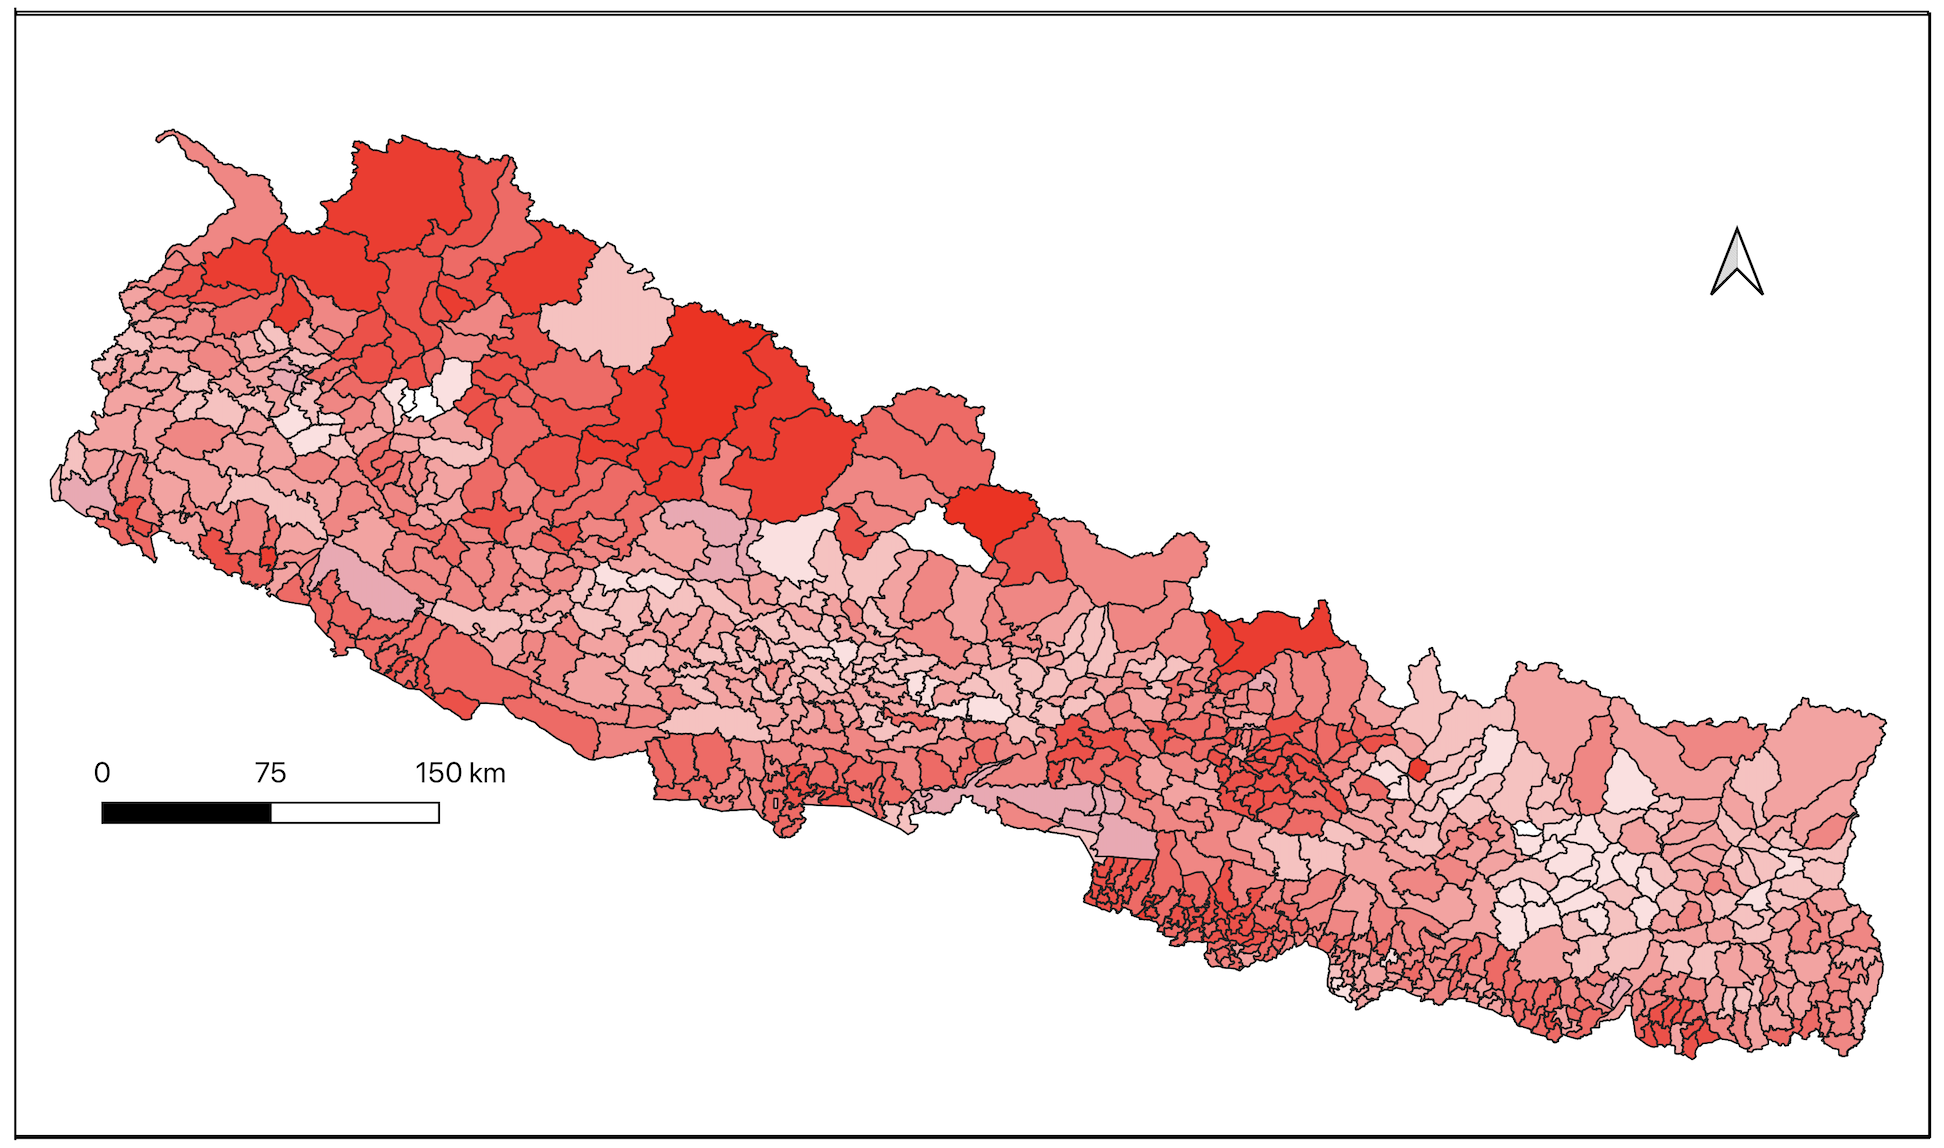
\includegraphics[width = 170mm, scale = 0.38]{figure/vote1.png}
\caption{Heatmap of Voting Turnout at local levels}
\label{Heatmap of Voting turnout}
\end{figure}
\begin{figure}[hptb]
\centering
\hspace{-1.5cm}
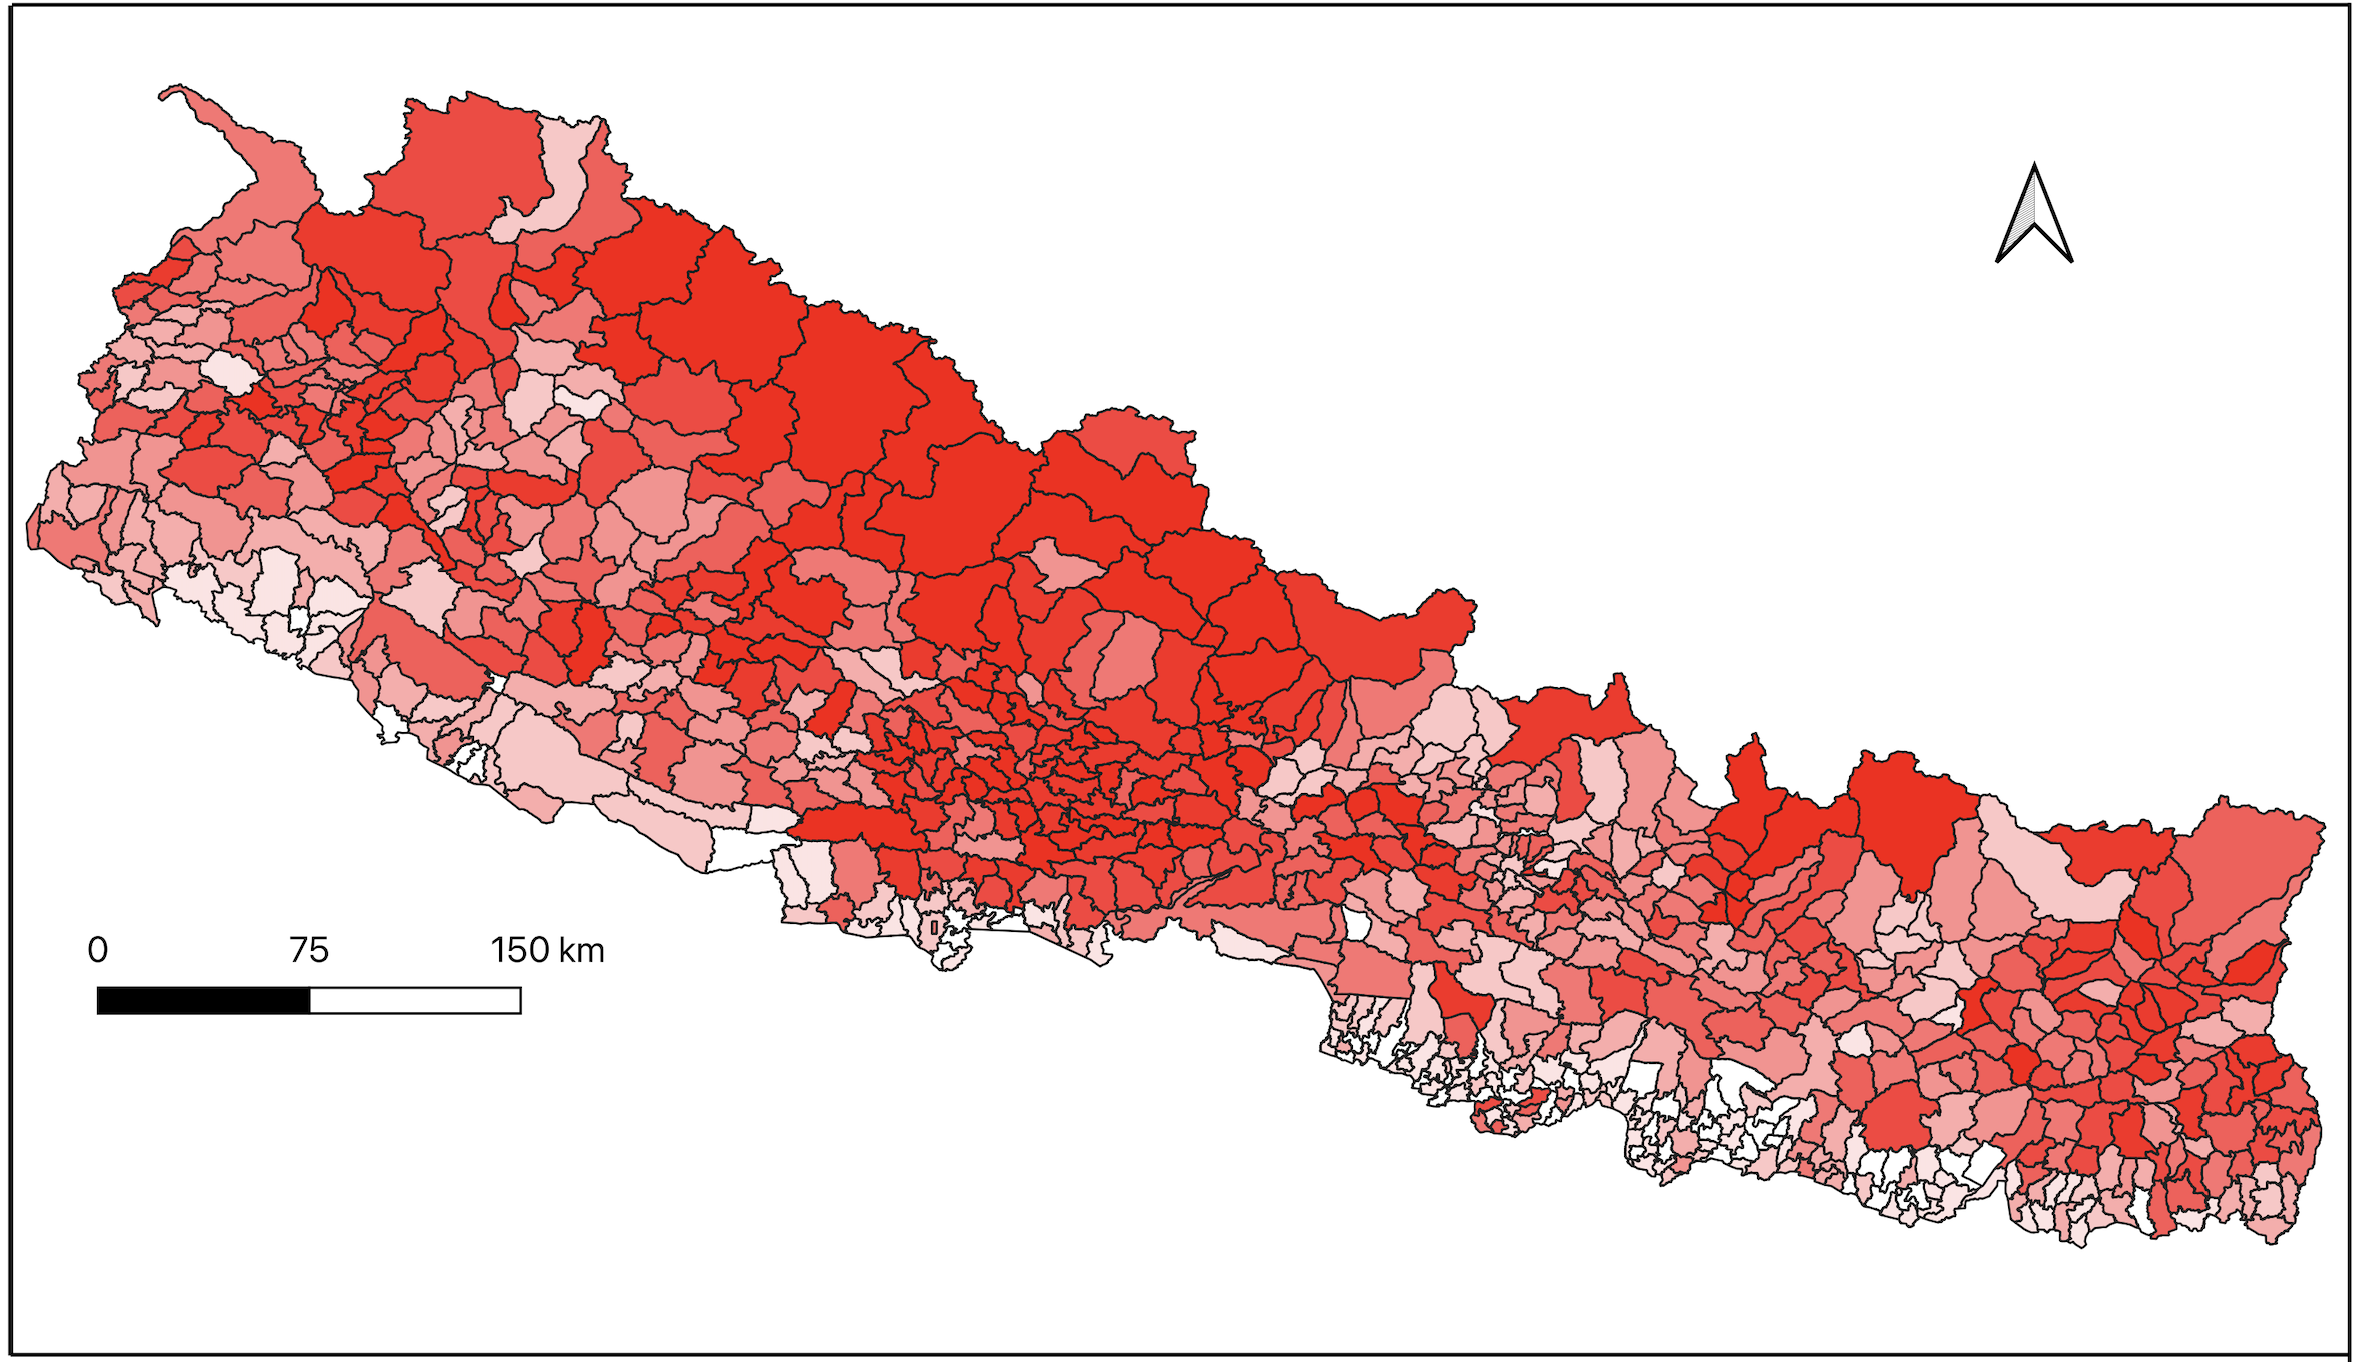
\includegraphics[width = 170mm, scale = 0.56]{figure/HHI.png}
\caption{Heatmap of Herfindahl-Hirschman Index}
\label{Heatmap of HH index}
\end{figure}
The difference between fiscal performances of local levels could have several determinants, including, structural and political characteristics\cite{Deborger1994}, neighbor local government effects\cite{Geys2006}, and voters involvement\cite{Geys2010}. Nepal's foray in federal system with proper power devolution provides an excellent opportunity to investigate the prime determinants of fiscal and economic discipline of local level units. While there exists seven provinces, acting as the intermediate governance mechanism between local levels and the central government, local level governments are closer to people and provides a better avenue to compare the performances across nation. Thus, the fiscal and economic performances of local level jurisdictions  are measured and their determinants are examined here instead of provincial level government. 
\subsection{Statement of the Problems}
In federal structure, local level governments are designed to be the closest accessible government to the general public. With the considerable administrative power wielded by the local governments of Nepal, their role is paramount in increasing the living standards of the denizens of the local levels. However, some jurisdictions have been able to provide the required services and perform their duties so as to increase the living standards relative to other jurisdictions that have fell behind. Existing disparities as well as the workings of the local level governments that could worsen the economic equity in the future is detrimental to the general welfare of the denizens as well as for the practice of federalism. The trend of economic disparities among local level governments goes against the spirit of the federalism, constitution, as well as against the principles of equality. With the massive effort and cost of restructuring the nation already incurred, the inequality in development across local level governments, caused by the fiscal and economic management, raises serious questions towards the economic and the political system of the nation. \\
As the fiscal and economic performances vary among the local levels, it is important to investigate the chief determinants of such variation. As people's will and mandate was paramount in installing the federal system of governance, the impact of electoral influence, an extension of people's will, on fiscal and economic performance must be examined. As fiscal and economic powers are devolved from the central government and are utilized by the local level governments, it should be employed in an accountable manner so as to minimize rent-seeking and shirking behaviors. Elections, through sanctioning and selection mechanism, strives to limit such behaviors and it is of critical importance to judge the effect elections could have on such behaviors.  \\
Election system in democracy offers the winner the authority to rule while simultaneously offering the loser the chance to run in the future\cite{Przeworski1999}. As elections are a medium to hold the elected officials accountable to the general public, electoral influence, through voting behaviors, influences the fiscal and economic working of the local level government of Nepal. Economic literatures are conflicting in the intensity and magnitude of effect electoral outcomes have on the fiscal and economic performances of the sub-national governments, thus, it is important to gauze what impact, on fiscal performance, did the first ever elected local government had in  Nepal.  \vspace{-3mm}
\subsection{Research Questions}
Based on the statement of the problem of this study, the research question are formulated. Thus, to properly analyze the differences in the electoral characteristics that led to differences in local level fiscal management, leading to some having a sound fiscal positions than others, the research question for this study could be stated as:
\begin{enumerate}[label=\roman*.]
    \item What are the differences in the electoral characteristics of  local level units of Nepal? 
    \item What are the differences in the fiscal performances of the local level governments of Nepal?
    \item How the differences in electoral characteristics translates to the differences in the fiscal performance of local level entities of Nepal?
 \end{enumerate}
 These are the fundamental research questions that this study aims to investigate and answer. The primary focus would be on the third question, i.e., how are electoral characteristics and fiscal performance of the local level governments are related. As based on the statement of problem these research questions were formed, based on the premises of these research questions, the objectives of the study is defined. \vspace{-4mm}
\subsection{Objectives of the Study}
The chief aim of this study is to investigate the determinants and the differences in fiscal performances among the local level governments of Nepal, potentially leading to inequality in taking development initiatives as well as unequal outcome in living standards. The electoral composition and involvement of the local level entities are also analyzed, especially in relation to its effect on the fiscal management by the elected officials. Thus, the specific objectives could be stated as:\\
I.\hspace{3mm} To analyze whether local electoral composition and behavior influence local government's performance in bevy of areas.  \\
II.\hspace{3mm} To gauge the impact of local government performance on economic and fiscal outcomes.\\
Additionally, apart from these two prime objectives, the accountability relationship that exists between the elected officials and  the electorate is also the objective of this study. \vspace{-3mm}
\subsection{Significance of the Study}
The purpose of this study is to understand the inherent as well as overtime evolved fiscal and economic differences in the local level. Federal structure with powerful local entities are new facet through which the developmental activities desired by people could be efficiently and effectively achieved. Thus, it is imperative that the workings of the federal structure and the differences among and within local levels be properly investigated. Differences in fiscal management, resulting in unequal development leads to constricted economic opportunities for the less developed regions in the future, increase the political discontent, as well as severely impact social wellbeing factors\cite{Saey1998} \\
The findings of this study would be useful in understanding if the federal system is working as intended for most of the populace. It will equally be useful in contextualizing the factors that are making some local levels different than others, and the ways of mitigating those factors. Similarly, this study could be useful in understanding how the grants and other economic assistance programs from the central governments should be diverted or targeted towards for better effectiveness.\\
Chiefly, this study contextualizes how accountable are the local elected representatives of Nepal to their electorate. The accountability aspect would be measured through the fiscal performances and the differences in such performances would be analyzed through the differences in electoral compositions, behaviors, and outcomes. As the federal system of governance is a recent development in Nepal, it is of extreme importance to gauze how the elected officials of the local level governments are fulfilling their economic and fiscal accountabilities to the denizens of their local level. 
\subsection{Limitations of the Study}
This study intends to use secondary data on economic activities of local levels to gauze their fiscal and economic differences. Those data in many cases were published by the local levels themselves or derived through the report of the AG office or through NNRFC. Similarly, the chief focus of this study is in economic sense, whereas the differences in local levels might be of non-economic in nature. Considering these factors, the chief limitations of this study can be summarized as:\\
i. \hspace{3mm} The secondary data to be collected, published by the local levels themselves, sometimes are presented without the audit from the AG office or the third party. Thus, those data might have inconsistencies and presents problems for this study.\\
ii.\hspace{3mm} The COVID-19 crises altered the financial and economic landscape of the local levels, with some suffering severely while other local levels were relatively unbothered.\\ 
iii.\hspace{3mm} The first election for the local level governments in 2017 were held in three distinct stages, from May to September. The results of the previous stage might have influenced the subsequent electorate behavior. For simplicity, this study omits such influence.\\
iv.\hspace{3mm} The LISA scores used in the analysis is a self-reported scores of the local governments, although there are several checks in the program to ensure the scores matches the performance. \\
v.\hspace{3mm} This study omits the effect of potential gerrymandering of local level governments. Gerrymandering changes the dynamics of the effect that electorate have on elected officials and makes complex the analysis of electoral accountability, thus, this study assumes no gerrymandering was carried out. \vspace{-3mm}
\subsection{Outline of the Study} 
This study contains the preliminary parts, the main body, bibliography, and annex. The preliminary parts, preceding the main body, consist of several pages, including the declaration sheet, approval sheet, acknowledgement, table of contents, list of tables, list of figures, list of abbreviations, and abstract. The bibliography section follows the main body, and at the end of this study annex is appended. Followings are the contents of the main body section of this study:\\
\textbf{{Chapter 1}: \hspace{0.75mm} Introduction:}\hspace{3mm} This first chapter basically explains what this study is about and how it is conducted. This chapter is further divided into the following sections:  
\begin{enumerate}[label=\roman*.]  
     \item Background of the study
    \item Statement of the problems
    \item Research Questions
    \item Objectives of the study
    \item Significance of the study
    \item Limitation of the study
    \item Outline of the study
\end{enumerate}
\textbf{{Chapter 2}: \hspace{0.75mm}Review of Literatures:}\hspace{3mm} This chapter is concerned with the existing body of work substantially related to the topic of this study. Thus, this chapter critically examines the books, journal articles, reports, and other concerned materials as they relate to the electoral accountability and fiscal performance. This chapter is sub-divided into theoretical and empirical review of existing literatures, with national context review sub-section added within the empirical section.\\
\textbf{{Chapter 3}: \hspace{0.75mm}Research Methodology:}\hspace{3mm} This chapter explains in detail the research design and the methods used to collect and analyze data. This sections further explains the nature of variables, the population and sample, and sources of data.\\
\textbf{{Chapter 4}: \hspace{0.75mm}Data Presentation and Analysis:}\hspace{3mm} This chapter details the nature and behavior of the data based on the framework of the preceding chapter. \\
\textbf{{Chapter 5}: \hspace{0.75mm}Summary, Conclusion, and Recommendations:}\hspace{3mm} This chapter summarizes the major findings of the research and presents the conclusion drawn, along with the suggested recommendations based on the results. 
